\documentclass[traditabstract]{aa} 
\input Planck.tex

% This is useful to overcome a bug in some versions of
% Adobe Acrobat for Windows
\pdfminorversion=4

\usepackage[breaklinks,colorlinks,citecolor=blue]{hyperref}
\usepackage{amsmath}
\usepackage{natbib}
\usepackage{graphicx}
\usepackage{txfonts}
\usepackage{natbib}
\usepackage{fixltx2e}

\graphicspath{{images/}{../python/figures/}{../IDL/IDL\_figures/}}

\newcommand{\sometext}{Text text text text text text text text text text text text text text text text text text text text text text text text text text text text text text text text text text text text text text text text text text text text text text text text text text text text text text text text text text text text text text text text text text text text text text text text text text text text text text text text text text text text text text text text text text text text text text text text text text text text text text text text text text text text text text text text text text text text text text text text text text text text text text text text text text text text text text text text text text text text text text text text text text text text text text text text text text text text text text text text text text text text text text text text text text text text text text text text text text text text text text text text text text text text text text text text text text text text text text text text text text text text text text text}

\bibpunct{(}{)}{;}{a}{}{,}

\begin{document}

\title{Figures for \Planck\ papers}
\subtitle{Examples and scripts}

\authorrunning{Figures for \Planck\ Papers}
\titlerunning{Examples and scripts}

\date{\today}

\abstract{Sample scripts are available that demonstrate how to produce figures compliant with the \Planck\ Style Guide in PGPLOT, IDL, and Python.}

\keywords{cosmic microwave background -- Instrumentation: polarimeters -- Methods: data analysis}

\maketitle

%%%%%%%%%%%%%%%%%%%%%%%%%%%%%%%%%%%%%%%%%%%%%%%%%%%%%%%%%%%%%%%%%%%%%%

\section{Introduction}
\label{sec:introduction}

Section~16 of the \Planck\ Style Guide gives general guidelines for figures in \Planck\ papers.  Unfortunately, the default settings of standard plotting packages do not produce figures compliant with these guidelines.  To help in the production of compliant figures, we have developed scripts that drive PGPLOT, IDL, and Python appropriately and can be adapted to the specific figures in \Planck\ papers.   These scripts and the figure files that they produce are available at

\url{http://github.com/zonca/paperplots/}

There is no text and therefore a lot of white space on many of the following pages.   We include \begin{verbatim}\clearpage\end{verbatim} after each set of figures to force them onto the page rather than let La\TeX\ decide how to rearrange them for more ``optimum'' placement.  

\def\fcaption{Comparison of the joint power spectrum estimates from the three CBI mosaics with the measurements from BOOMERANG, DASI, and MAXIMA. The rectangles indicate the 68\% confidence intervals on band-power; for BOOMERANG, the solid rectangles indicate the 68\% confidence interval for the statistical and sample variance errors, while the hatched rectangles shows the amount by which a $\pm1\sigma$ error in the beamwidth ($12\farcm9 \pm 1\farcm4$) would shift the estimates (all up or all down together). The {\it black curve} is the joint model (see text).}



\section{Line plots}

The most common type of figure is the line plot.  Plots of the same data are shown below made by PGPlot, IDL, and Python.  


$\vec{A}$ and
$\tens{B}$


\subsection{PGPlot}

Figures~1--3 show the same data plotted by PGPlot for the three sizes of figure that A\&A uses, single-column (88\,mm), side-caption (120\,mm), and two-column (180\,mm).  In each case, adjustments are made so that the letters, numbers, and characters in the axis labels remain 1.9--2.0\,mm in height.


% Single-column figure

\begin{figure} 
  \includegraphics[width=\hsize]{aafig_1cropped.pdf}
  \caption{\fcaption} 
  \label{line_pgplot88}
\end{figure}


% Figure with side caption

\begin{figure*} 
  \sidecaption
  \includegraphics[width=12cm]{aafig_2cropped.pdf} 
  \caption{\fcaption} 
  \label{line_pgplot120}
\end{figure*}


% Two-column figure

\begin{figure*} 
  \includegraphics[width=18cm]{aafig_3a_resized_cropped.pdf}
  \caption{\fcaption} 
  \label{line_pgplot180}
\end{figure*}

The required LaTeX commands are

\begin{verbatim}
\begin{figure} % Single-column figure
  \includegraphics[width=\hsize]{f13.eps}
  \caption{\fcaption} 
  \label{line_pgplot88}
\end{figure}

\begin{figure*} % Figure with side caption
  \sidecaption
  \includegraphics[width=12cm]{f13.eps} 
  \caption{\fcaption} 
  \label{line_pgplot120}
\end{figure*}

\begin{figure*} % Two-column figure
  \includegraphics[width=17cm]{f13.eps}
  \caption{line_pgplot180} 
  \label{fig2col}
\end{figure*}
\end{verbatim}



\clearpage






\subsection{IDL}

The three equivalent figures as produced by IDL are shown in Figs.~4--6.

\begin{figure}[h]
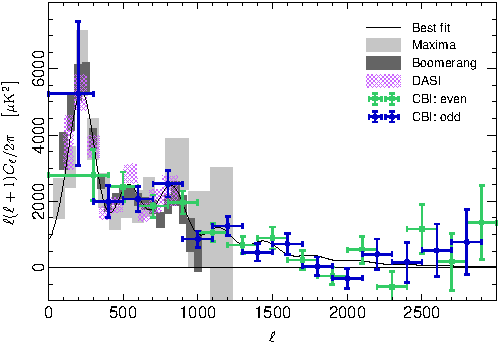
\includegraphics[width=8.8cm]{PlanckFig_lineplot_IDL_88mm.pdf}
\caption{\fcaption} 
\end{figure}

\begin{figure*}
\sidecaption
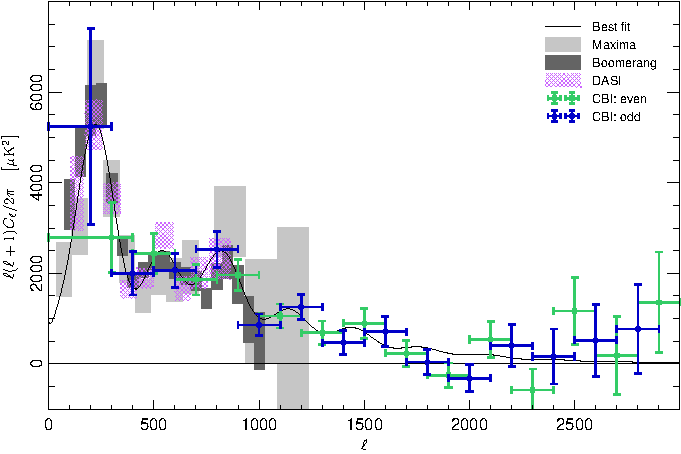
\includegraphics[width=12cm]{PlanckFig_lineplot_IDL_120mm.pdf}
\caption{\fcaption}
\end{figure*}

\begin{figure*}
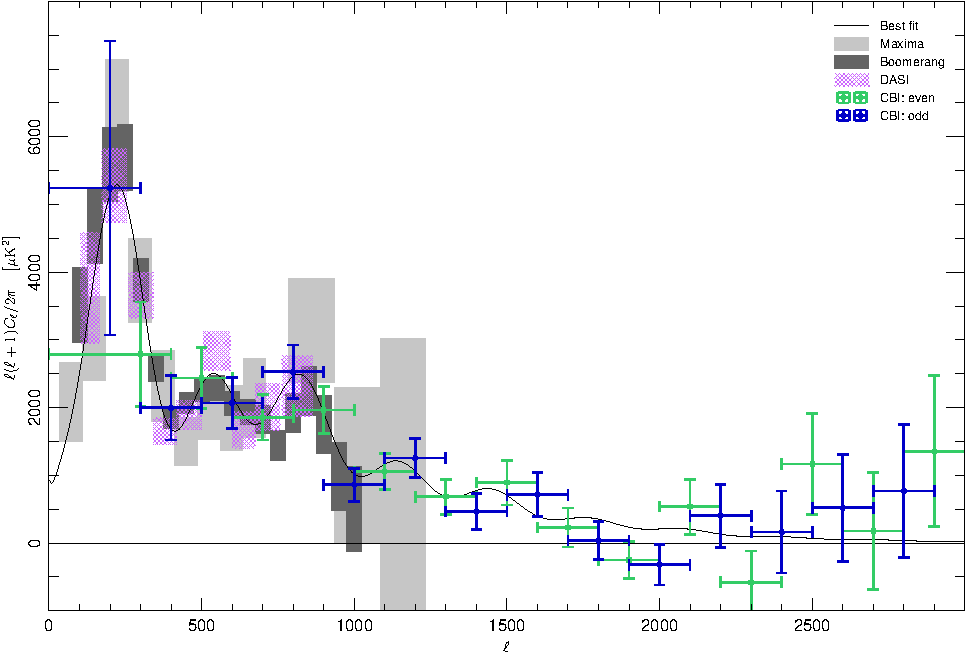
\includegraphics[width=18cm]{PlanckFig_lineplot_IDL_180mm.pdf}
\caption{\fcaption}
\end{figure*}

\clearpage

IDL scripts are also given for two-panel (top, bottom) figures.  Here's what they look like.


\begin{figure}[h]
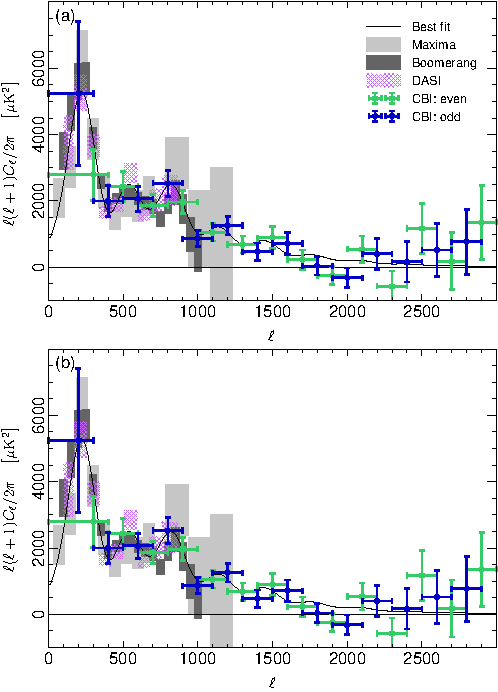
\includegraphics[width=8.8cm]{PlanckFig_lineplot_IDL_2x88mm.pdf}
\caption{\fcaption} 
\end{figure}

\begin{figure*}
\sidecaption
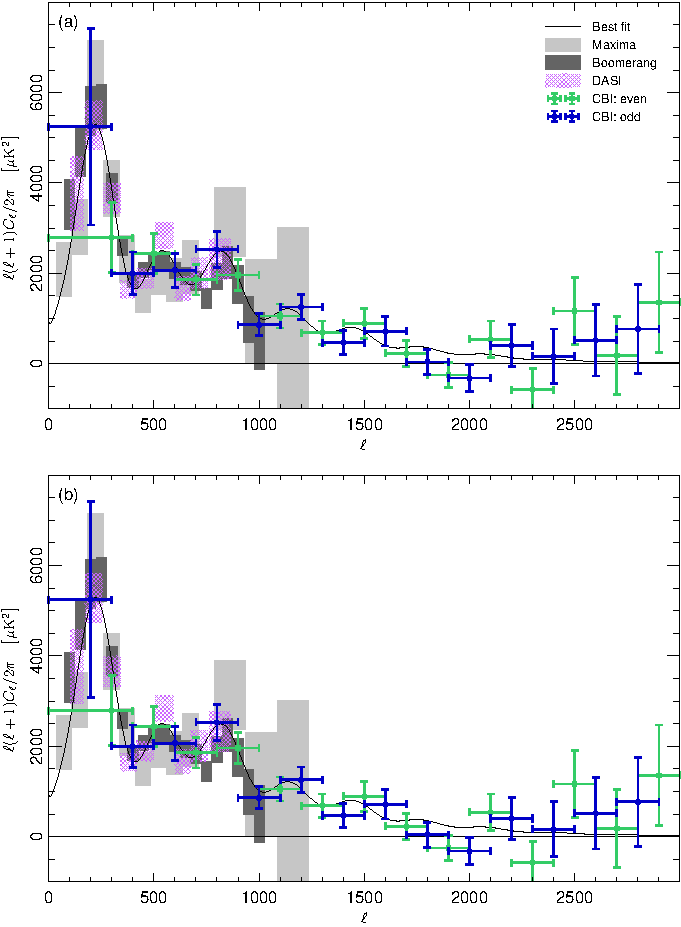
\includegraphics[width=12cm]{PlanckFig_lineplot_IDL_2x120mm.pdf}
\caption{\fcaption}
\end{figure*}

\begin{figure*}
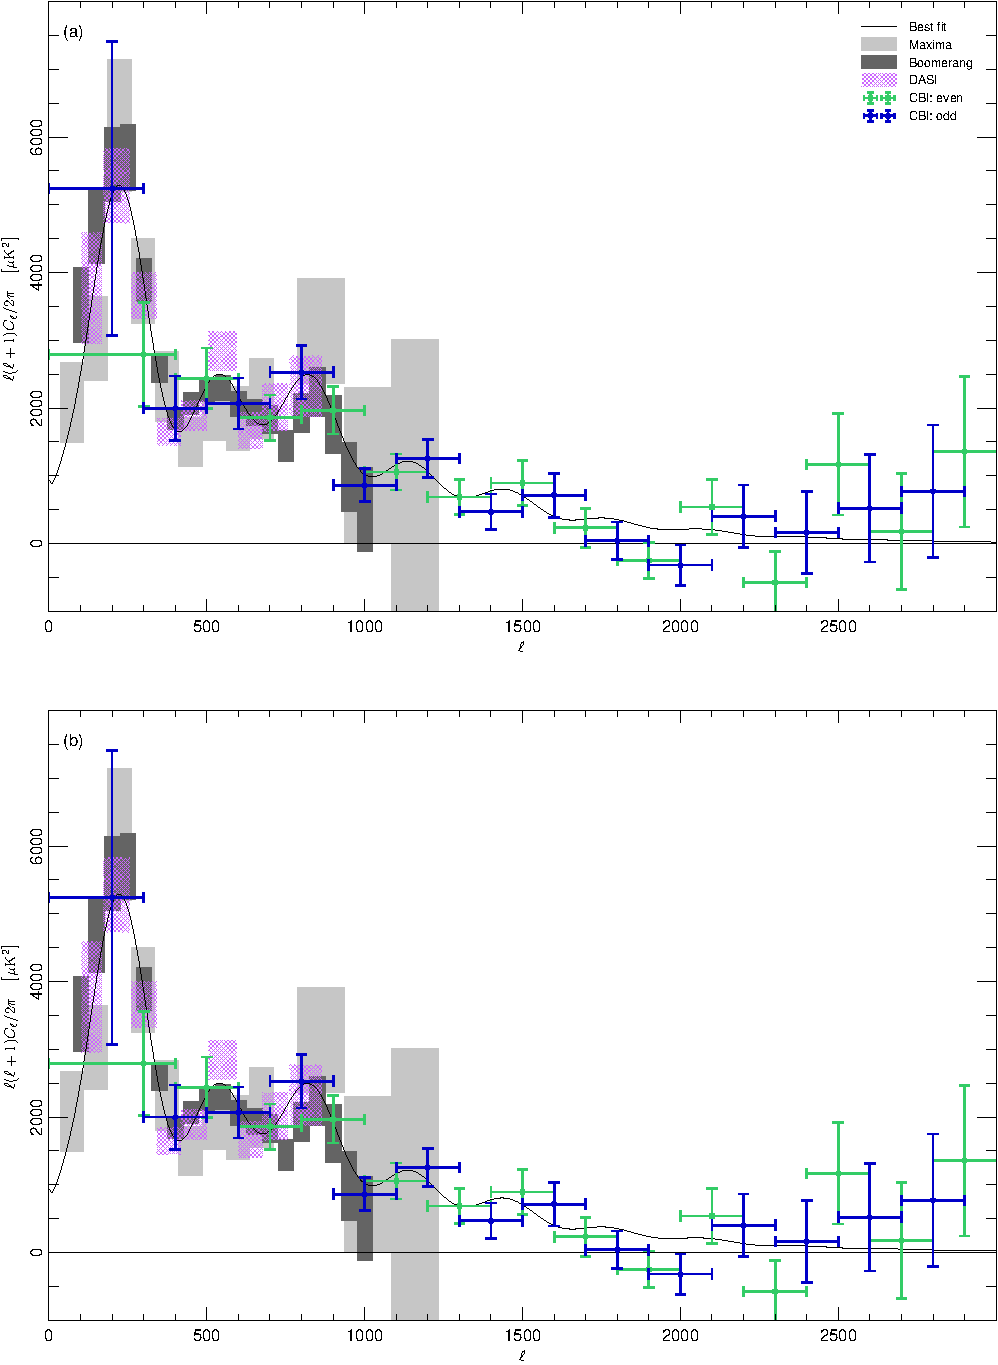
\includegraphics[width=16.8cm]{PlanckFig_lineplot_IDL_2x180mm.pdf}
\caption{This two-panel figure is taller than the A\&A page when the width is set to 180\,mm.  The width has been reduced so that it fits.}%\fcaption}
\end{figure*}

\clearpage





\subsection{Python}

The three equivalent figures as produced by Python are shown in Figs.~7--9.


\begin{figure}[ht]
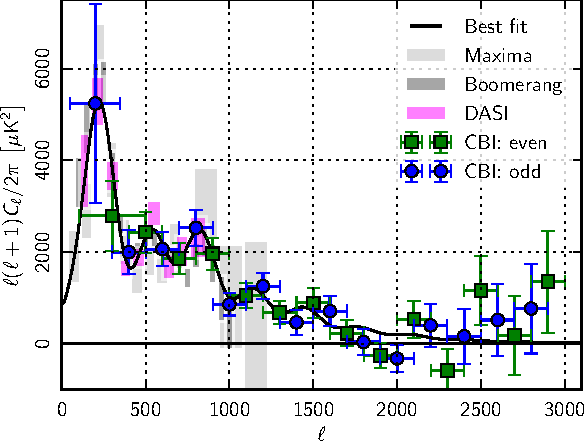
\includegraphics[width=8.8cm]{PlanckFig_lineplot_python_88mm.pdf}
\caption{\fcaption} 
\end{figure}


\begin{figure*}[ht]
\sidecaption
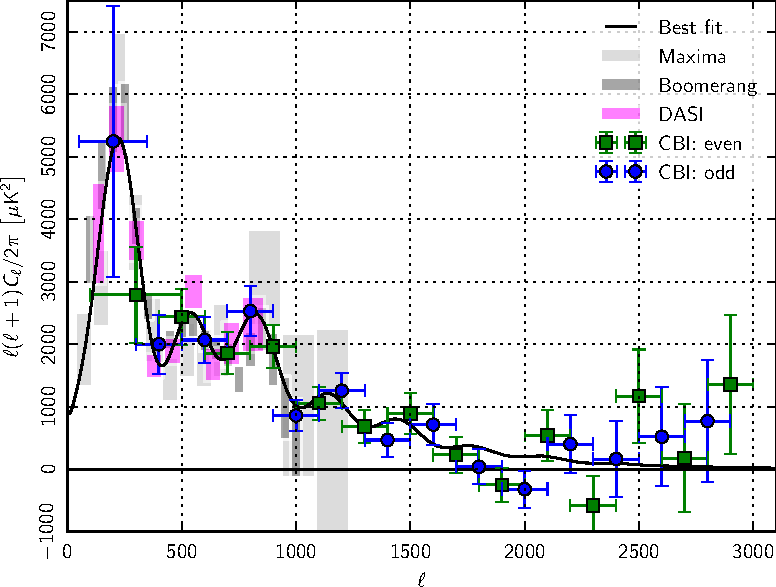
\includegraphics[width=12cm]{PlanckFig_lineplot_python_120mm.pdf}
\caption{\fcaption}
\end{figure*}

\begin{figure*}[t]
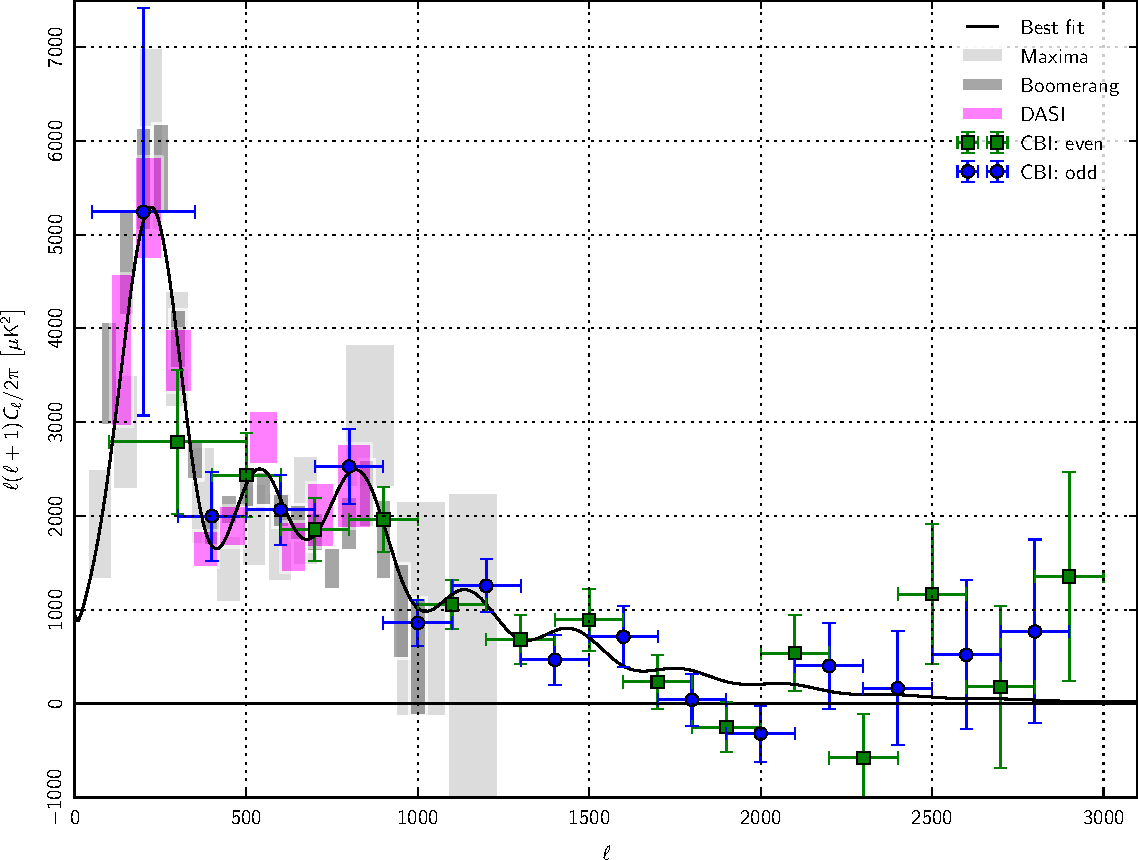
\includegraphics[width=18cm]{PlanckFig_lineplot_python_180mm.pdf}
\caption{\fcaption}
\end{figure*}

\clearpage











\section{Maps}

An example map is shown in the three standard sizes, and also with two different colour tables.  Do not, \textit{ever}, change the aspect ratio of a Mollweide projection by specifying both height and width or by any other means.  The geometric properties of the projection are destroyed.  


\subsection{Python}


\begin{figure}[ht]
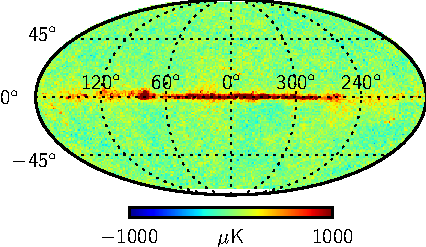
\includegraphics[width=8.8cm]{PlanckFig_map_python_88mm}
\caption{Mollview, 88\,mm wide.  The map itself is bitmapped, but all text is vectorized.} 
\label{fig:map_python88} 
\end{figure}

\begin{figure}[ht]
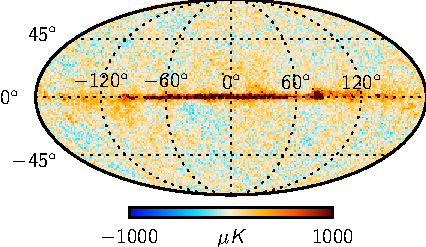
\includegraphics[width=8.8cm]{PlanckFig_map_colombi1_python_88mm}
\caption{Mollview, 88\,mm wide.  The map itself is bitmapped, but all text is vectorized.} 
\label{fig:map_parchment_python88}
\end{figure}



\begin{figure*}[ht]
\sidecaption
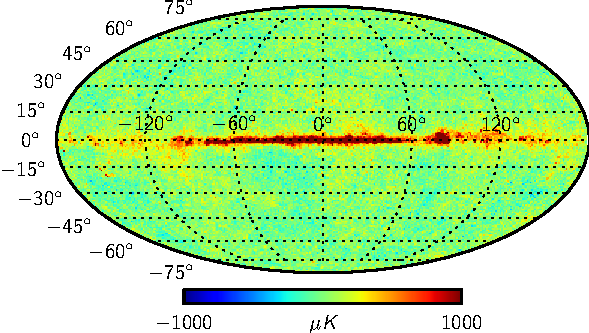
\includegraphics[width=12cm]{PlanckFig_map_python_120mm}
\caption{Mollview, 120\,mm wide.  The map itself is bitmapped, but all text is vectorized.}
\label{fig:map_python120} 
\end{figure*}

\begin{figure*}[ht]
\sidecaption
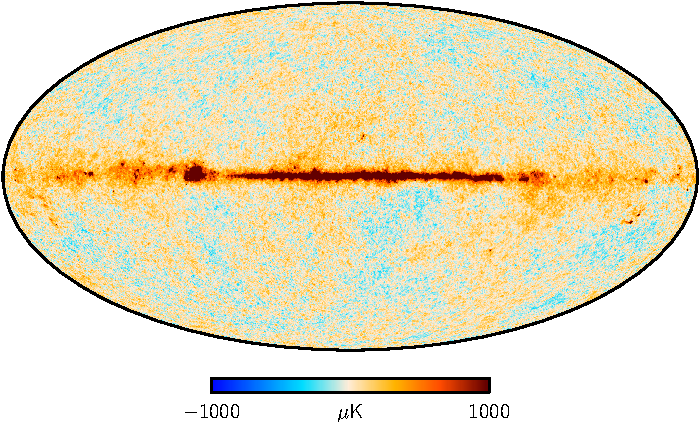
\includegraphics[width=12cm]{PlanckFig_map_colombi1_python_120mm}
\caption{Mollview, 120\,mm wide.  The map itself is bitmapped, but all text is vectorized.} 
\label{fig:map_parchment_python120}
\end{figure*}



\begin{figure*}[H!b]
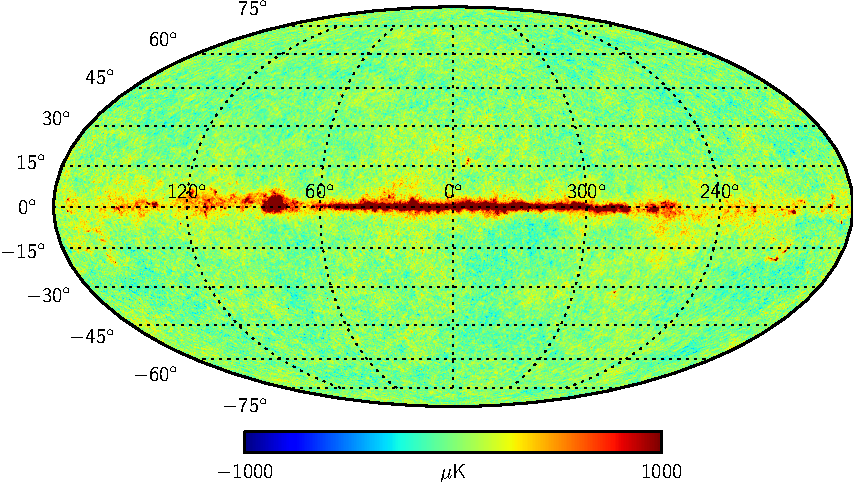
\includegraphics[width=18cm]{PlanckFig_map_python_180mm}
\caption{Mollview, 180\,mm wide.  The map itself is bitmapped, but all text is vectorized.}
\label{fig:map_python180}
\end{figure*}


\begin{figure*}[H!b]
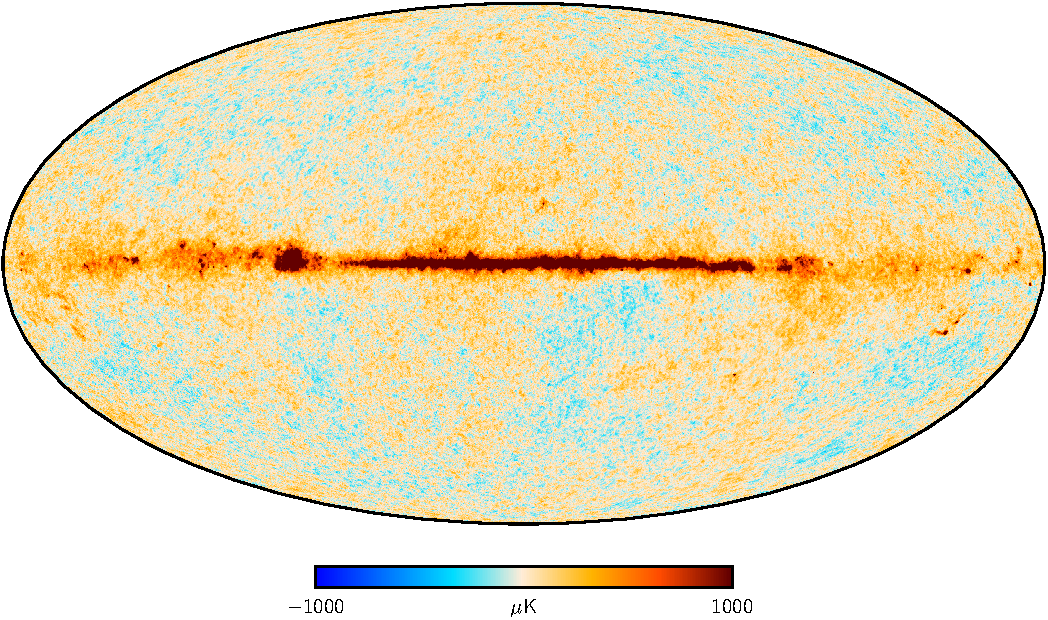
\includegraphics[width=18cm]{PlanckFig_map_colombi1_python_180mm}
\caption{Mollview, 180\,mm wide.  The map itself is bitmapped, but all text is vectorized.}
\label{fig:map_parchment_python180}
\end{figure*}


\clearpage


\subsection{IDL}



\begin{figure}[ht]
\includegraphics[width=8.8cm]{PlanckFig_map_colombi1_IDL_88mm}
\caption{Mollview, 88\,mm wide.  The map itself is bitmapped, but all text is vectorized.} 
\label{fig:map_parchment_python88}
\end{figure}




\begin{figure*}
\sidecaption
\includegraphics[width=12cm]{PlanckFig_map_colombi1_IDL_120mm}
\caption{Mollview, 120\,mm wide.  The map itself is bitmapped, but all text is vectorized.} 
\label{fig:map_parchment_python120}
\end{figure*}



\begin{figure*}[H!b]
\includegraphics[width=18cm]{PlanckFig_map_colombi1_IDL_180mm}
\caption{Mollview, 180\,mm wide.  The map itself is bitmapped, but all text is vectorized.}
\label{fig:map_parchment_python180}
\end{figure*}


\clearpage



\section{Parameter-type plots}

\subsection{Python}


\begin{figure}[ht]
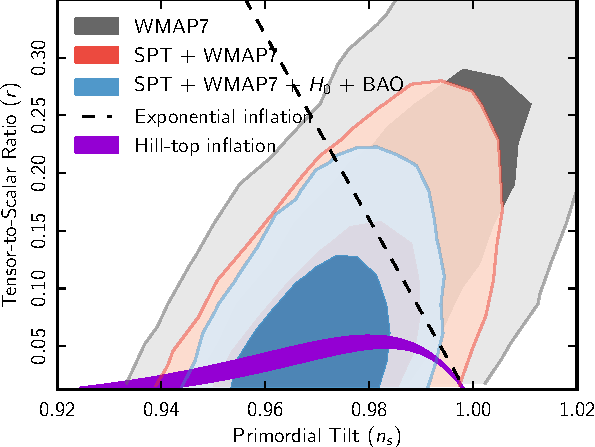
\includegraphics[width=\columnwidth]{PlanckFig_parameters_python_88mm}
\caption{Parameters, 88\,mm wide.  The use of transparency is essential for clarity.}
\label{fig:parameters_python88}
\end{figure}

\begin{figure*}[H!b]
\sidecaption
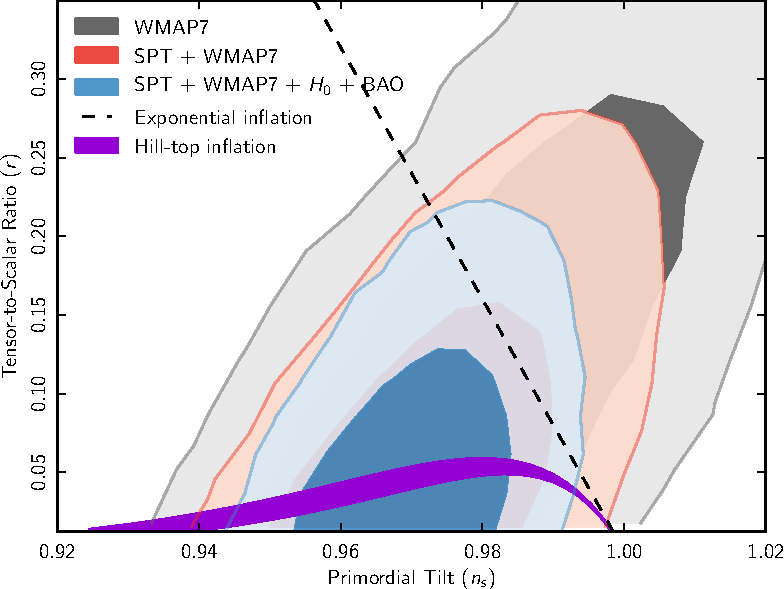
\includegraphics[width=12cm]{PlanckFig_parameters_python_120mm}
\caption{Parameters, 120\,mm wide.  The use of transparency is essential for clarity.}
\label{fig:parameters_python120}
\end{figure*}

\begin{figure*}[H!b]
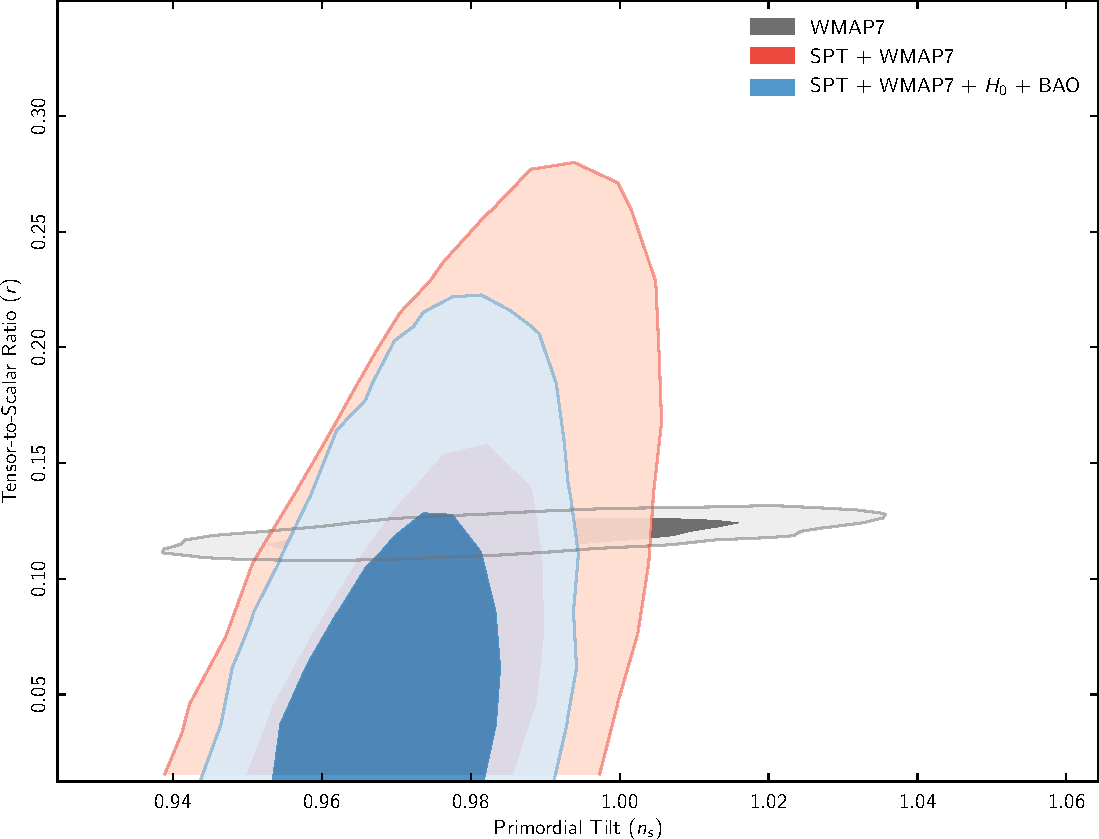
\includegraphics[width=18cm]{PlanckFig_parameters_python_180mm}
\caption{Parameters, 180\,mm wide.  The use of transparency is essential for clarity.}
\label{fig:parameters_python180}
\end{figure*}

\clearpage


\section{Linewidth tests}

The next page shows the same plot made with six different specified line thicknesses
in IDL, as indicated.  If the page is displayed at large size or on a high
resolution screen, the line thicknesses vary smoothly as expected.  Printed at A4 size, they depend significantly on the resolution of the printer, with quantized variations that are somewhat unpredictable.  Try printing the next page and see what happens.  If a line thickness needs to be specified (defaults are most likely OK), use 0.15--0.20\,mm (call it 0.5\,pt).  

\clearpage

\begin{figure}
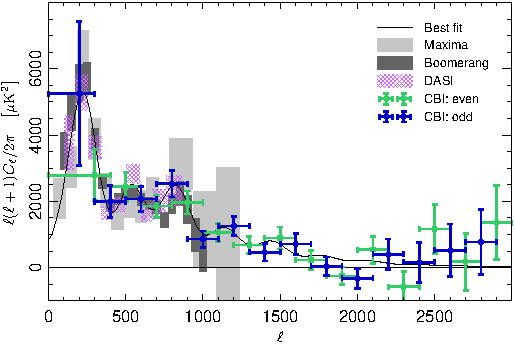
\includegraphics[width=\columnwidth]{PlanckFig_lineplot_IDL_88mm_0_10mm_lines}
\caption{Linewidth 0.10\,mm.}
\label{fig:parameters_python88}
\end{figure}


\begin{figure}
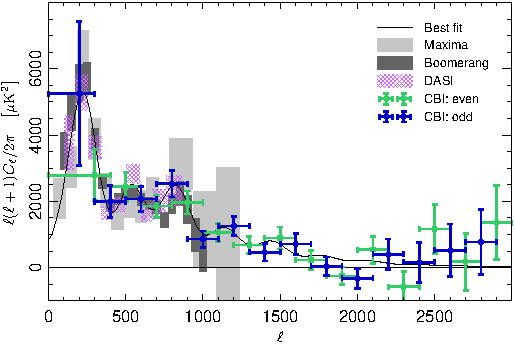
\includegraphics[width=\columnwidth]{PlanckFig_lineplot_IDL_88mm_0_15mm_lines}
\caption{Linewidth 0.15\,mm.}
\label{fig:parameters_python88}
\end{figure}



\begin{figure}
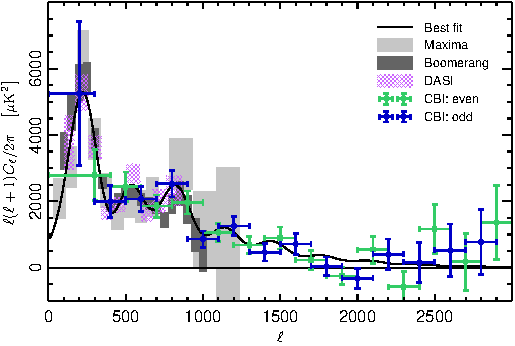
\includegraphics[width=\columnwidth]{PlanckFig_lineplot_IDL_88mm_0_20mm_lines}
\caption{Linewidth 0.20\,mm.}
\label{fig:parameters_python88}
\end{figure}



\begin{figure}
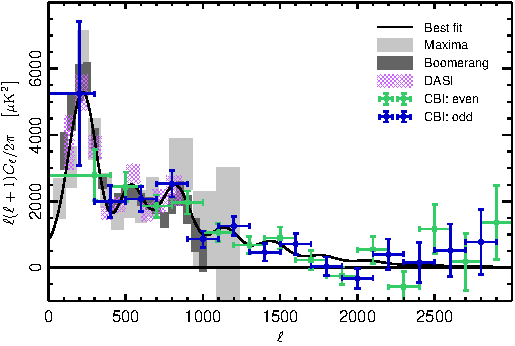
\includegraphics[width=\columnwidth]{PlanckFig_lineplot_IDL_88mm_0_25mm_lines}
\caption{Linewidth 0.25\,mm.}
\label{fig:parameters_python88}
\end{figure}



\begin{figure}
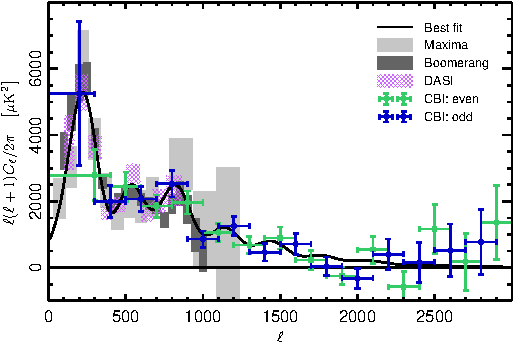
\includegraphics[width=\columnwidth]{PlanckFig_lineplot_IDL_88mm_0_30mm_lines}
\caption{Linewidth 0.30\,mm.}
\label{fig:parameters_python88}
\end{figure}



\begin{figure}
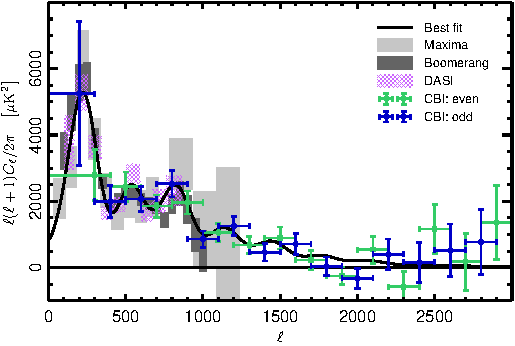
\includegraphics[width=\columnwidth]{PlanckFig_lineplot_IDL_88mm_0_35mm_lines}
\caption{Linewidth 0.35\,mm.}
\label{fig:parameters_python88}
\end{figure}








\end{document}




20\pdeg8 21\pdeg8 22\pdeg8 23\pdeg8 24\pdeg8 25\pdeg8 26\pdeg8 27\pdeg8 28\pdeg8 29\pdeg8

20\fdg8 21\fdg8 22\fdg8 23\fdg8 24\fdg8 25\fdg8 26\fdg8 27\fdg8 28\fdg8 29\fdg8

20\parcm8 21\parcm8 22\parcm8 23\parcm8 24\parcm8 25\parcm8 26\parcm8 27\parcm8 28\parcm8 29\parcm8

20\farcm8 21\farcm8 22\farcm8 23\farcm8 24\farcm8 25\farcm8 26\farcm8 27\farcm8 28\farcm8 29\farcm8

20\parcs8 21\parcs8 22\parcs8 23\parcs8 24\parcs8 25\parcs8 26\parcs8 27\parcs8 28\parcs8 29\parcs8

20\farcs8 21\farcs8 22\farcs8 23\farcs8 24\farcs8 25\farcs8 26\farcs8 27\farcs8 28\farcs8 29\farcs8

